\documentclass{article}
\usepackage[margin=1in]{geometry}
\usepackage{graphicx}
\usepackage{listings}
\usepackage{url}

\author{Iúri Figueiredo Archer}
\date{\today}
\title{Documentation zum VRML Projekt\\\large{Computergrafik WS21/22}}


\begin{document}
\maketitle
\section*{Einleitung und Werkzeuge}
Dieses Dokument dient sowohl als Dokumentation für die Abgabe wie auch
als meine eigene Referenz um die Abgabe zu erleichtern. Desweiteren
nutze ich die Gelegenheit auch um meine \LaTeX\ Kenntnisse zu
erfrischen.

Es wurden folgende Programme benutzt, um das VRML Projekt zu
realizieren.
\begin{itemize}
\item \textit{Visual Studio Code} für VRML und Python
\item \LaTeX\ für die Dokumentation
\item \textit{view3dscene} und \textit{Cortona3D} für die
Visualisierung der VRML-Welt
\item \textit{draw.io} wurde für das Erstellen der Diagramme und
Skizzen genutzt und um diese als .pdf zu exportieren.
\end{itemize}

\textit{Cortona3D} war leider notwendig, da \textit{view3dscene} noch
keine Skripte unterstützt (weder JS noch VRML-Script). 
Dies stellte sich als Herausforderung, da Cortona3D nur von Internet
Explorer unterstützt wird und sonst keinem anderen Browser - was mir
als Linux Nutzer besonders viel Spaß bereitet hat.

Dieses Projekt wurde mit Git erstellt und existiert als
Repository auf Github unter \url{github.com/cyberme0w/VRMLProjekt}.




\newpage

\section{Aufgaben und Umfang der Bearbeitung}
\subsection*{V1}
\subsubsection*{a)}
Die Szene wurde im VRML-Browser \textit{view3dscene} geöffnet, da es
leider für Linux keine vernünftige Alternative gibt. 

\subsubsection*{b)}
Das entsprechende Szenengraph sieht folgendermaßen aus:

\begin{figure}[!!h]
    \centering
    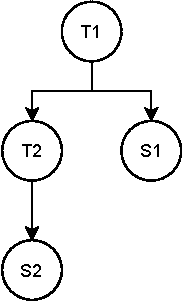
\includegraphics{V1_SceneGraph.pdf}
    \caption{Szenengraph aus \textit{Transform}- und \textit{Shape}-Knoten von meinErstesVRML.wrl}
\end{figure}


\subsubsection*{c)}
Ändert man die Rotation oder Translation von T1 (oberstes Transform), wirkt 
diese auf beide Figuren (Sphere und Box). Ändert man die untergeordnete
Transforms, wirken diese nur auf die entsprechende Figur. Die Eigenschaft
scaleOrientation gibt an, bezogen auf welche Axe die Skalierung durchgeführt
wird. Da in der meinErstesVRML Welt keine Skalierungen durchgeführt werden, 
spielt die scaleOrientation keine Rolle.

\subsubsection*{d) (Zusatzaufgabe)}
Man kann die \textit{Shapes} einfärben, indem man eine der \textit{Color}
Eigenschaften des Material Knoten verändert. 

\begin{lstlisting}[language=VRML]
#VRML V2.0 utf8
material Material{ diffuseColor 0  1 0 } # Green
material Material{ diffuseColor 1 .65 0 } # Orange
\end{lstlisting}




\newpage 

\subsubsection*{e) (Zusatzaufgabe)}
\begin{figure}[!ht]
    \centering
    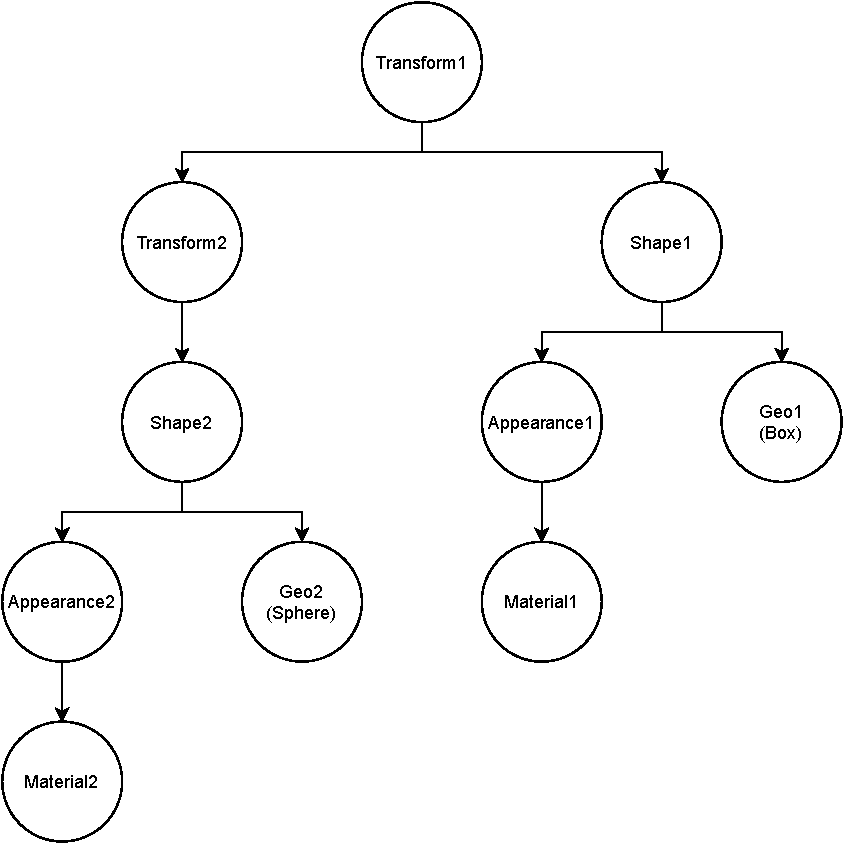
\includegraphics[scale=0.5]{V1_fullSceneGraph.pdf}
    \caption{vollst. Szenengraphen von meinErstesVRML.wrl}
\end{figure}

\subsection*{V2}
\subsubsection*{a)}
Es wurde anhand der vorhandenen Punkte folgende Skizze erstellt:

\begin{figure}[!h]
    \centering
    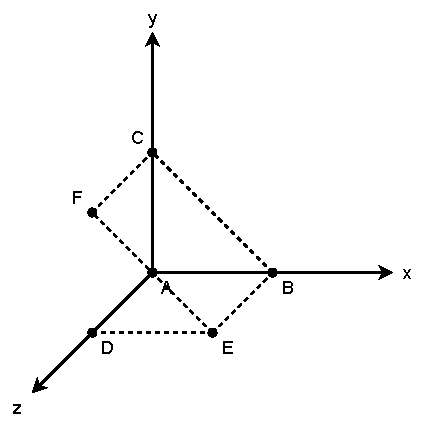
\includegraphics{V2_Sketch.pdf}
    \caption{Skizze zu \textit{meinZweitesVRML.wrl} anhand der Punkte}
\end{figure}

Die Szene wurde anschließend im VRML-Browser \textit{view3dscene} geöffnet, da es
leider für Linux keine vernünftige Alternative gibt.

\subsubsection*{b)}
Die Standardblickrichtung von view3dscene ist:
\begin{itemize}
    \item POS: 0.50 0.50 3.00
    \item DIR: 0.00 0.00 -1.00
    \item UP: 0.00 1.00 0.00
\end{itemize}

Man sieht aus dieser Richtung nichts, weil nur die Rückseiten der Flächen
sichtbar sind. Wenn man \textbf{solid false} wieder "reinkommentiert",
werden die Flächen nicht mehr als Teile eines Körpers mit Volumen (wo die
Innenseiten nicht dargstellt werden müssen) betrachtet und daher werden
die Rückseiten auch dargestellt.

"The solid field indicates whether the shape encloses a volume (TRUE), and
 can be used as a hint to perform backface culling. If nothing is known
 about the shape, this field value is FALSE (and implies that backface culling
 cannot be performed and that the polygons are two-sided)."
 
 Quelle (11.11.2021):
 
 \url{http://graphcomp.com/info/specs/sgi/vrml/spec/part1/concepts.html#GeometryNodes}

\subsubsection*{c)}
Aufgabe in der Datei erledigt. Siehe \textit{meinZweitesVRML.wrl}.

\subsubsection*{d)}
Der Mittelpunkt des Vierecks BCFE ist [0.5 0.5 0.5].

\subsubsection*{e) und f) (Zusatzaufgaben)}
Beide Aufgaben wurden in \textit{meinZweitesVRML.wrl} erledigt.

\begin{figure}[h]
    \centering
    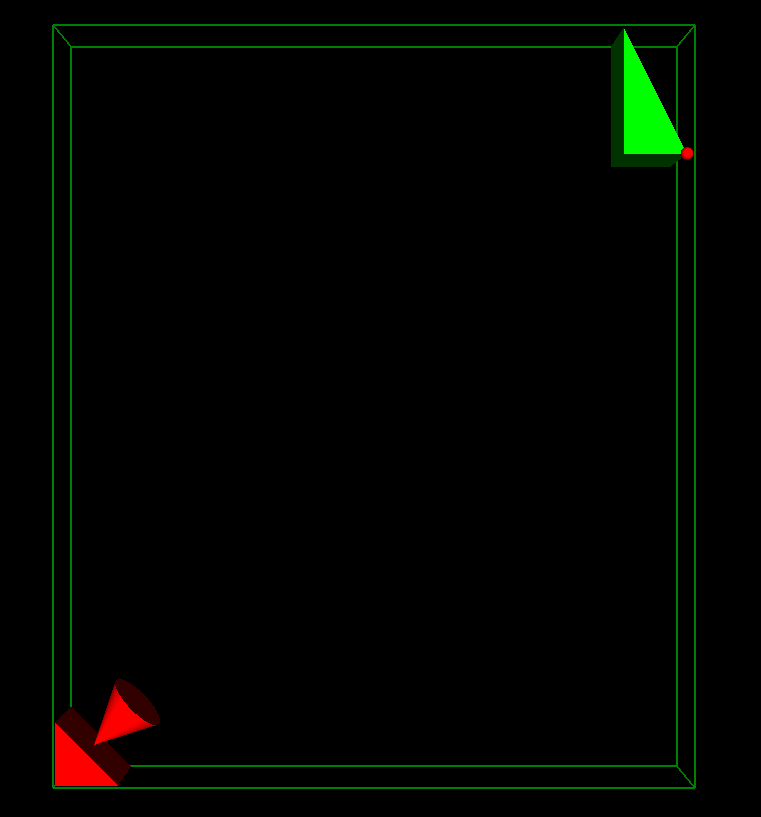
\includegraphics[scale=0.375]{V2_e_und_f.png}
    \caption{Das gleiche Prisma mit verschiedenen Eigenschaften. Die rote Kugel dient als Hilfspunkt.}
\end{figure}




\newpage

\section*{Das eigentliche VRML Projekt}
Nicht jede Aufgabe ab hier benötigt eine Beschreibung, da die Arbeit aus der Visualisierung der .wrl
Datei genügen dürfte. Hier eine Liste der Aufgaben, die erledigt wurden.

\begin{itemize}
    \item V3:
    \begin{itemize}
        \item a) Datei anlegen - \textbf{DONE}
        \item b) Skifahrer - \textbf{DONE}
        \item c) Berghang - \textbf{DONE}
        \item d) Skifahrer zu Proto - \textbf{DONE}
    \end{itemize}
    \item V4:
    \begin{itemize}
        \item a) Vogelperspektive - \textbf{DONE}
        \item b) 4 weitere Viewpoints - \textbf{DONE}
        \item c) FPV Skifahrer + Name - \textbf{DONE}
    \end{itemize}
    \item V5:
    \begin{itemize}
        \item a) Grüne Scheinwerfer - \textbf{DONE}
        \item b) (Zusatz) Lichtkegel - \textbf{DONE}
    \end{itemize}
    \item V6:
    \begin{itemize}
        \item a) Skybox - \textbf{DONE}
        \item b) Scheinwerfer AN/AUS Skript - \textbf{DONE}
    \end{itemize}
    \item V7:
    \begin{itemize}
        \item a) Skifahrer Animation (Gerade + Kreis) - \textbf{DONE}
        \item b) Klick auf Skifahrer für Animation -\textbf{DONE}
        \item c) Schlitten verfolgt Skifahrer
    \end{itemize}
    \item V8:
    \begin{itemize}
        \item a) Kastenhaus + Baum Texturen - \textbf{DONE}
        \item b) Nachtskifahren + Fackel - \textbf{DONE}
    \end{itemize}
    \item V9 (Zusatz): Verschönerungen - \textbf{DONE}
\end{itemize}




\newpage

\subsection*{Anmerkungen zu den Aufgaben}
\subsubsection*{V3b}
Für das Anlegen des Skifahrers wurde zuerst eine Skizze erstellt, um die
Verbindung der Punkte im indexedFaceSet zu vereinfachen. Da ich dieses Kunstwerk
mit der Welt teilen möchte, füge ich es hier mal ein. Dies entspricht nicht das
Endergebnis, welches in \textit{miniproject.wrl} zu sehen ist. Das Objekt besteht
außerdem aus mehr als 50 Oberflächen, allerdings wurde dies in Rücksprache mit
Herrn Dörner gemacht und soll kein Problem darstellen.

\begin{figure}[h]
    \centering
    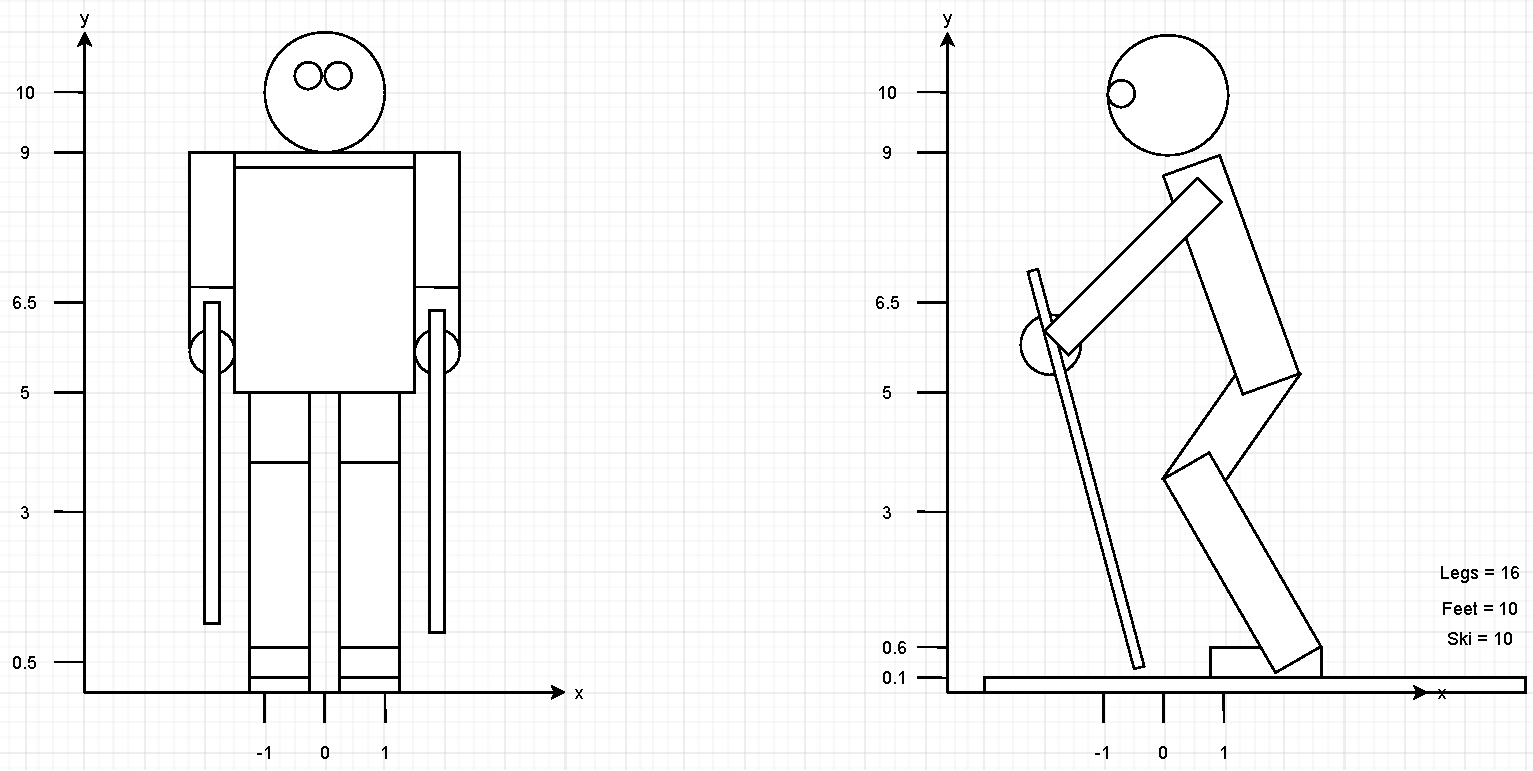
\includegraphics[scale=0.5]{skifahrer_sketch.pdf}
    \caption{Erste Skizze des Skifahrers}
\end{figure}

\subsubsection*{V9}
Es wurden zwei Verschönerungen durchgeführt. folgendes gemacht:

Die erste Verschönerung besteht aus einer innerhalb des Hauses integrierte Werbewand.
Die soll eher als Easter Egg gesehen werden, als ernsthafter Versuch, die Szene 
deutlich schöner zu machen. Ich hoffe, ich kann dennoch hiermit zeigen, dass ich
in VMRL mit Video-Dateien umgehen kann, wie in der Aufgabe gefordert.

Die zweite Verschönerung war die Verbesserung der Skifahrt auf kurvengenauen Pfaden.
Die Punkte wurden mit einem selbstgeschriebenen Pythonskript ausgerechnet und können
somit beliebig genau sein. Die Datei ist ebenfalls im Ordner enthalten.

\begin{lstlisting}[language=Python]
    import numpy as np
    import math as m
    
    def calculatePointsWithinAngle(ammount, centerX, centerY, radius, startTime, endTime, startAngle, endAngle):
    
        # calculate increments and create array
        angleIncrement = (endAngle - startAngle) / (ammount + 1)
        timeIncrement = (endTime - startTime) / (ammount + 1)
        points = np.zeros((ammount + 2, 4), dtype=float)
    
        # calculate each point
        for i in range(ammount + 2):
            currentAngle = startAngle + angleIncrement * i
            currentTime = startTime + timeIncrement * i
            
            # x value
            points[i][0] = centerX + radius * m.cos(m.radians(currentAngle))
    
            # y value
            points[i][1] = centerY + radius * m.sin(m.radians(currentAngle))
            
            # rotation (depending on clockwise/counterclockwise)
            if(angleIncrement > 0):
                points[i][2] = m.radians(currentAngle + 90)
            else:
                points[i][2] = m.radians(currentAngle - 90)
    
            # time
            points[i][3] = currentTime
    
        return points
    
    def printVRMLfromPoints(points):
    
        print("\npositions:")
        print("key [")
        for point in points:
            print("{:.5f}".format(point[3]))
        print("]")
        print("keyValue [")
        for point in points:
            print("{:.2f} {:.2f} {:.2f}".format(point[0], 0.0, point[1]))
        print("]")
    
        print("\norientations:")
        print("key [")
        for point in points:
            print("{:.5f}".format(point[3]))
        print("]")
        print("keyValue [")
        for point in points:
            print("0 1 0 {:.2f}".format(point[2]))
        print("]")

    # Beispieleingabe
    center = (-48.5, 282)
    radius = 23.5
    ammount = 10
    startTime = 0.23
    endTime = 0.30
    startAngle = 0
    endAngle = -90
    
    points = calculatePointsWithinAngle(ammount, center[0], center[1], radius, startTime, endTime, startAngle, endAngle)
    printVRMLfromPoints(points)
\end{lstlisting}





\newpage 

\section*{Quellen und Lizenzen}
\subsubsection*{Texturen}
\begin{itemize}
    \item Brick Texture, von bart:
        \begin{itemize}
            \item Datum: 29.11.2021
            \item \url{https://opengameart.org/content/brick-texture}
            \item Lizenz: CC-BY 3.0 + CC-BY-SA 3.0 + GPL 3.0
        \end{itemize}
    \item Baumstamm, von bart:
        \begin{itemize}
            \item Datum: 29.11.2021
            \item \url{https://opengameart.org/content/seamless-tiling-tree-bark-texture}
            \item Lizenz: GPL 2.0 + GPL 3.0 + CC-BY-SA 3.0
        \end{itemize}
    \item Baumblätter, von qubodup:
        \begin{itemize}
            \item Datum: 29.11.2021
            \item \url{https://opengameart.org/content/wall-grass-rock-stone-wood-and-dirt-480}
            \item Lizenz: CC0
        \end{itemize}
    \item Door, von qubodup:
        \begin{itemize}
            \item Datum: 29.11.2021
            \item \url{https://opengameart.org/content/weathered-wood-door}
            \item Lizenz: CC-BY 3.0
        \end{itemize}
    \item Never Gonna Give You Up (video clip)
        \begin{itemize}
            \item Datum: 30.11.2021
            \item \url{https://www.youtube.com/watch?v=iik25wqIuFo}
            \item Lizenz: ehm... Fair Use?
        \end{itemize}
\end{itemize}
\end{document}
